% !TeX encoding = UTF-8
% !TEX root = ./presentation.tex
\section{Metodologia a ser Executada}
   \subsection{Design\ Referencial de Software\ Utilizando Grafo de Controle de Fluxo}
      \begin{frame}{Design\ de Sistemas Embutidos}
         \begin{itemize}  \setlength{\itemsep}{1.6em}
            \item Fundamentos para o compreendimento do particionamento;
            \item Metodologia baseada em \parencite{Sass2010, Arato2003, Arato2005, Mann2007, Hassine2017}.
         \end{itemize}
      \end{frame}
   
      \begin{frame}{Grafo de Controle de Fluxo (GCF)} \vspace{-1em}
         \begin{itemize}
            \setlength{\itemsep}{1.2em}
            \item Por que utilizá-lo:
            \begin{itemize}
               \item \textbf{Descrever um sistema}, tanto em \software\ ou \hardware, \textbf{livre de uma especificação} de forma
               \item Rápidos protótipos, referenciado como \design\ de referência de \software\ (DRS).
            \end{itemize}
   
            \item O sistema inicial é dado como \textbf{grafo de tarefas/rotinas}, define-se \bx{$ C = (B, F) $} onde
            \begin{description}
               \item [$B$:] vértices que representam os blocos básicos; e 
               \item [$F$:] arestas que indicam a todas as possibilidades de caminhos entre os blocos.
            \end{description}
         \end{itemize}
      \end{frame}
   
      \begin{frame} %\vspace{-1em}
         \begin{figure}[h] \centering
            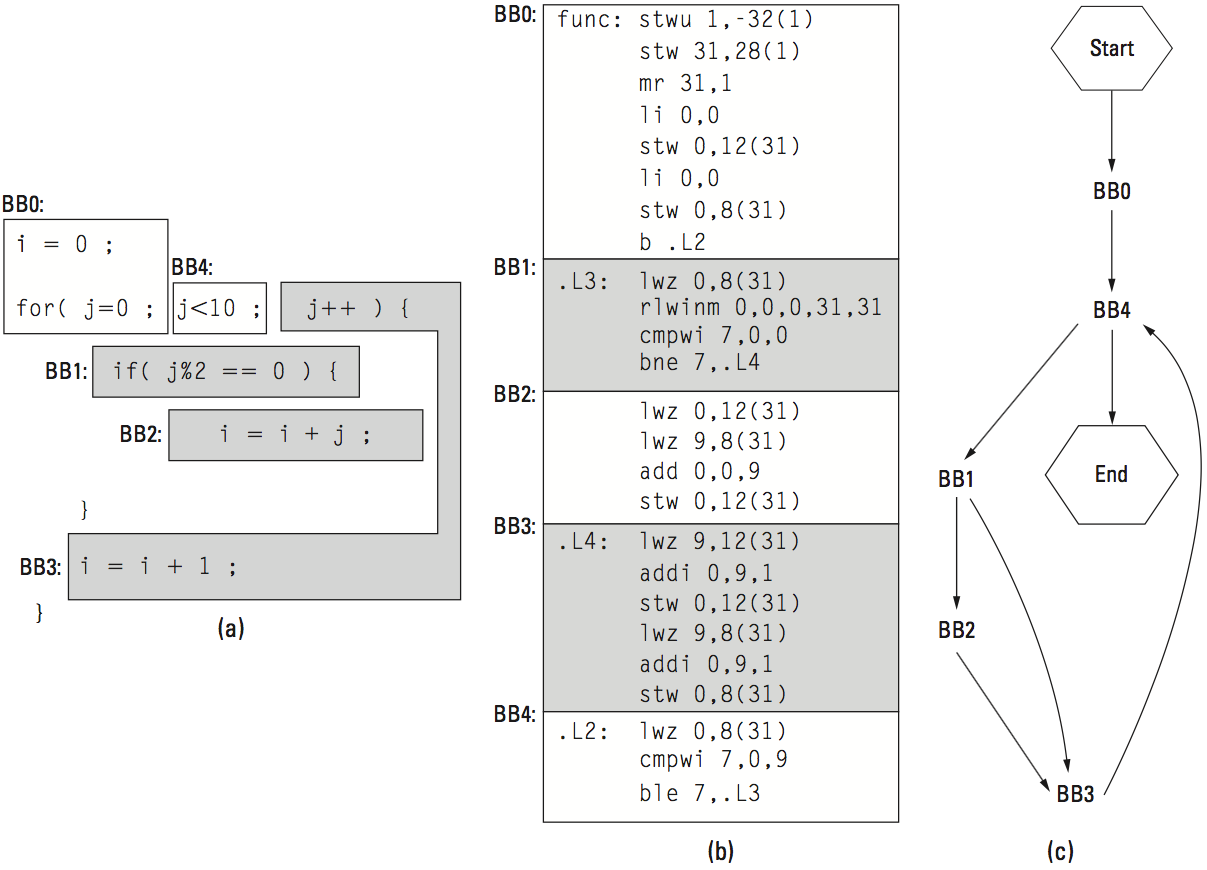
\includegraphics[width=0.89\textwidth]{img/f3-6.png}
            \caption{Identificação de blocos básicos e a representação de cada modelo de descrição de \software.}
            %\label{fig:f3-6}
         \end{figure}
      \end{frame}
   
   \subsubsection{Grafo de Chamada (GC)}
   
      \begin{frame}{Grafo de Chamada (GC)}
         %Modelado uma sub-rotina de um DRS utilizando o GCF, define-se o Grafo de Chamada (GC).
   
         \begin{itemize}
            \setlength{\itemsep}{0.6em}
            \item \textbf{Consiste num conjunto de Grafos de Controle de Fluxo}, um por sub-rotinas, ou seja
               \bx{$\mathcal{C} = {C_0, C_1, \dots C_{n-1}}$}
            onde 
            \begin{description}
               \item[$ C_i = (B_i, F_i) $:] \textbf{representa o GCF de uma sub-rotina} $ i $.
            \end{description}
   
            \item Grafo estático de chamada da aplicação é \bx{$\mathcal{A} = (\mathcal{C}, \mathcal{L}) \label{eq:a}$} onde
            \begin{description}
               \item [\A:] representa uma aplicação específica; e
               \item [$ \mathcal{L} \subseteq \mathcal{C} \times \mathcal{C} $:] plano cartesiano das invocações de rotinas.
            \end{description}
   
         \end{itemize}
   
         \begin{block}{Duas sub-rotinas são relacionadas se}
            Podem ser determinadas, no tempo de compilação, que a \textbf{sub-rotina $ i $ tem potencial de invocar a sub-rotina $ j $}, ou seja, \bx{$ (C_i, C_j) \in \mathcal{L} $}.
         \end{block}
         \pdfnote{Para entendimento da partição}
         \pdfnote{um subconjunto do plano cartesiano dos GCF}
      \end{frame}
   
      \begin{frame}{Definição Formal de Partição}
   
         Uma partição $ \mathcal{S} = \{S_0, S_1, \dots\} $ de um conjunto universal $ U $ \textbf{é um conjunto de subconjuntos de} $ U $ sendo que
            %
            \begin{eqnarray}
               \bigcup_{S \in \mathcal{S}} S &=& U \label{eq:part_form_1} \\ \pause
               \forall S, S' \in \mathcal{S} | S \cap S' &=& \emptyset \label{eq:part_form_2} \\
               \forall S \in \mathcal{S} \cdot S &\neq& \emptyset \label{eq:part_form_3}
            \end{eqnarray}
            \pause
            Considere $ U = \{a, e, i, o, u, y\} $. Uma partição $ \mathcal{X}_i $ de $ U $:
            \begin{eqnarray}
            \mathcal{X}_a &=& \left\{\{a, e, i, o, u\}, \{y\}\right\} \label{eq:xa} \\
            \mathcal{X}_b &=& \left\{\{a\}, \{e\}, \{i\}, \{o\}, \{u\}, \{y\}\right\} \label{eq:part_a} \\
            \mathcal{X}_c &=& \left\{\{a\}, \{e\}, \{i\}, \{o\} \right\} \label{eq:part_c} \\
            \mathcal{X}_d &=& \left\{\{a, e, i\}, \{i, o, u, y\}, \{\}\right\} \label{eq:part_d}
            \end{eqnarray}
            
           \textit{$\mathcal{X}_c$ viola a Eq. 1, $\mathcal{X}_d$ viola Eqs. 2 e 3.}
            
         \pdfnote{1: cada ele d $ U $ é membro de 1+ $ S \in \mathcal{S} $}
         \pdfnote{2,3: S são emparelhados disjuntos e não vazio}
         \pdfnote{cada ele $ U $ termina em um dos $\mathcal{S}$ e nenhum dos s é vazios.}
      \end{frame}
   
   
   
   \subsection{Particionamento}
      \begin{frame}{Aplicar o Formalismo à Aplicação $\mathcal{A} = (\mathcal{C}, \mathcal{L})$}
         \begin{itemize}
            \item Assume-se que
            \begin{description}
               \item [Universo:] é o conjunto dos \textit{blocos básicos} $B$ de todas as sub-rotinas de um dispositivo \wearable;
               
               \item [$\therefore U$:] é as partições de sub-rotinas
            \end{description}
            
            %
            \begin{equation}
               U = \bigcup_{C \in \mathcal{C}} B(C) \label{eq:bigcup}
            \end{equation}
            ou seja, uma partição $\mathcal{S}$
            \begin{equation}
               \mathcal{S}  = \left \{
               \underbrace{\left \{ b_0, b_1, \dots, b_i \right \}}_{\text{sub-rotina }C_0},
               \underbrace{\left \{ b_i, b_{i+1}, \dots, \right \}}_{\text{sub-rotina }C_1},\dots
               \underbrace{\left \{ b_j, b_{j+1}, \dots, \right \}}_{\text{sub-rotina }C_{n-1}}
               \right \}
            \end{equation}
   
            \item Propósito
            \begin{enumerate}
               \item \textbf{Reorganizar a partição} de blocos básicos e então;
               \item \textbf{Mapear} cada subconjunto.
            \end{enumerate}
   
         \end{itemize}
      \end{frame}
   
   
   
      \begin{frame}{Aplicar o Formalismo à Aplicação $\mathcal{A} = (\mathcal{C}, \mathcal{L})$}
         \begin{itemize}  \setlength{\itemsep}{0.6em}
            \item Dessa forma pode-se
            \begin{itemize}
               \item Criar e remover subconjuntos \textbf{não vazios};
               \item Mover blocos básicos ao redor até ter uma nova partição.
            \end{itemize}
   
            \item $\therefore \mathcal{A}’ = (\mathcal{C}’, \mathcal{L}’) $, inferido a partir da reorganização da partição $ \mathcal{X}’ $.
   
               \bigskip
   
            \item Em seguida, mapeia-se cada subconjunto de $ \mathcal{X} $ para ambos \hs
   
         \end{itemize}
            { \footnotesize
            \begin{equation}
               \mathcal{X}'   = \left \{
               \underbrace{
                  \underbrace{
                     \left \{ b_j, b_{j+1}, \dots, \right \}
                  }_{\text{sub-rotina }C_k}
                  \underbrace{
                     \left \{ b_k, b_{k+1}, \dots, \right \}
                  }_{\text{sub-rotina }C_l}
                  \dots
               }_{\text{\software}}
               \
               \underbrace{
                  \underbrace{
                     \left \{ b_0, b_1, \dots, b_i \right \}
                  }_{\text{sub-rotina }C_r}
                  \underbrace{
                     \left \{ b_i, b_{i+1}, \dots, \right \}
                  }_{\text{sub-rotina }C_s}
                  \dots
               }_{\text{\hardware}}
               \right \} \label{eq:part_final}
            \end{equation}
            }
      \end{frame}
   
   
   
   \subsection{Ganho de Performance}
   
      \begin{frame}{Ganho de Performance} \vspace{-1em}
         \begin{itemize} \setlength{\itemsep}{1.0em}
            \item \textbf{\Software:} Análise de ordem de complexidade;
            \item \textbf{\Hardware:} Não possui um guia geral para comparação, e por isso utiliza-se ganho de performance.
   
            \item Definições prévias
            \begin{description} \setlength{\itemsep}{0.4em}
               \item [$ s(i) $:] tempo de execução esperado para uma invocação de uma sub-rotina $ i $;
               \item [$ h(i) $:] tempo de execução em \hardware;
               \item [$ m(i) | i \in \mathcal{H} $:] aproximação do montante gasto na transferência de um estado ou o custo de configuração e latência;
               \item [$ \gamma $:] representa o ganho de performance (speedup), $ \gamma > 1.0 $.
            \end{description}
         \end{itemize}
      
         \begin{equation}
            \gamma(i) = \frac{s(i)}{h(i) + m(i)}
         \end{equation}
      \pdfnote{y = gamma}
      \end{frame}
   
   
      \begin{frame}{Ganho de Performance} \vspace{-1em}
         \begin{block}{Do que a aplicação depende para ter maior velocidade?}
            \textbf{Ganhos de performance do recurso} e o \textbf{quão frequentemente ele é utilizado} no \design\ referencial de \software.
         \end{block}
      
         \begin{itemize}
            \item \textbf{Fração do tempo de um recurso em \software}\ $ p(i) $ a partir de informações de \textit{profile}.
         \end{itemize}
            \vspace{-1em}
         \begin{eqnarray}
            %\gamma(i) & = & \frac{s(i)}{h(i) + m(i)} \\
            \Gamma & = & \left [
                                 (1 - p(i))
                                 +
                                 \frac{
                                    p(i)
                                 }{
                                    \gamma(i)
                                 } \right 
                              ]^{-1} \\
%            \Gamma & = & \left [
%                                 (1 - p(i))
%                                 +
%                                 \frac{
%                                    p(i)
%                                 }{
%                                    \frac{s(i)}{h(i) + m(i)}
%                                 } \right 
%                                 ]^{-1}
\Gamma (\mathbb{D}) & = &
\left [
1 + \sum _{i \in \mathbb{D}} \left (
\frac{
   p(i)
}{
   \gamma(i)
}-p(i)
\right)
\right ]^{-1}
         \end{eqnarray}
         
         \begin{description}
            \item [$\gamma(i)$:] performance individual de cada recurso (acelerador);
            \item [$p(i)$:] fração de tempo de um recurso particular (\software);
            \item [$\mathbb{D}$:] recursos em \hardware.
         \end{description}
         
         \pdfnote{Inversao: da taxa de execução p tempo de execução, mantendo o sentido de GanPerf.}
      
      \end{frame}
   
      \begin{frame}{Consideração de Recursos}
         \begin{itemize}
            \item Contar-se o número de células lógicas requeridas para cada recurso
         \end{itemize}
         \begin{description}
            \item [$ r_{FPGA} $:] total de números de células lógicas \textbf{disponíveis};
            
            \item [$ r(i) $:] quantidade de células lógicas \textbf{por cada recurso} $ i $.
         \end{description}
            
            \begin{eqnarray}
            \sum_{i \in \mathbb{D}} r(i) < r_{FPGA} & \quad \text{e} \quad & 
            \vec{r}_{FPGA} =
            \begin{pmatrix}
            r_{Logic\ Cells} \\
            r_{Memory}\\
            r_{DSP}\\
            \vdots \\
            r_{n-1}
            \end{pmatrix}
            \end{eqnarray}
            
            \begin{equation}
            \therefore \sum_{i \in \mathbb{D}} \vec{r}(i) < \vec{r}_{FPGA}
            \end{equation}
            
         \pdfnote{Implementar tudo em h ignorando custos de desenvolvimento/recursos.}
         \pdfnote{D é o conjunto de recurso no \design.}
         \pdfnote{rotas não sao calculadas}
      \end{frame}
      
      
   \subsection{A Proposta: Particionamento para Sistemas Wearable}

      \begin{frame}{Formulação do Problema para \Wearables}
         \begin{itemize}
            \item Definições
            \begin{description}
               \item [$ \mathbb{D} $:] todos os recursos em \hardware;
               \item [$ \mathbb{C} $:] conjunto candidatos;
            \end{description}
         
            \begin{equation}
            \begin{array}{rrcl}
            \text{max}                 & \Gamma ( \mathbb{D})               & ~   & ~                \\
            & & & \\
            subject\ to & \sum_{i \in \mathbb{D}} \vec{r}(i) & < & \vec{r}_{FPGA}
            \end{array}
            \label{eq:constraints}
            \end{equation}
            
               \bigskip
            
            \item Ou seja
      
            \begin{enumerate} \setlength{\itemsep}{0.6em}
               \item Encontrar todas as partições de $ U $;
               \item Sintetizá-las;
               \item \textit{Profiling};
               \item Avaliar quantitativamente cada $ \Gamma $.
            \end{enumerate}
         \end{itemize}
      \pdfnote{p gamma}
      \end{frame}
   
      \begin{frame}[fragile]
         \begin{figure}
            \begin{tikzpicture}[auto, node distance=2.5 cm, >=latex']
            %\tikzstyle{block}    = [draw, rectangle, minimum height=2em, minimum width=4em, fill=red!20]
            %\tikzstyle{input}    = [coordenate]
            %\tikzstyle{output}   = [coordenate]
            %\tikzstyle{pinstyle} = [pin edge={to-,thin,black}]
            \matrix[column sep = .75cm, row sep = .375cm]{
               & \node[draw, shape=rectangle, fill=red!20, visible on=<1->] (hl) {High Level Source}; & \\
               & \node[draw, shape=rectangle, fill=red!20, visible on=<2->] (profile)    {Profiling}; & \\
               & \node[draw, shape=rectangle, fill=red!20, visible on=<3->] (candidate) {Gets Candidates};& \\
               \node[draw, shape=rectangle, fill=red!20, visible on=<4->] (soft) {Software Compiler}; & & 
               \node[draw, shape=rectangle, fill=red!20, visible on=<4->] (hard) {Hardware Synth}; \\
               & \node[draw, shape=rectangle, fill=red!20, visible on=<5->] (evaluate) {Evaluates it};  & \\
               & \node[draw, shape=rectangle, fill=red!20, visible on=<6->] (solve) {Solved};  & \\
            }; 
            \draw [->, thick, visible on=<1->] (hl) -- (profile);
            \draw [->, thick, visible on=<2->] (profile) -- (candidate);
            \draw [->, thick, visible on=<3->] (candidate) -- node {Non Candidates} (soft) ;
            \draw [->, thick, visible on=<3->] (candidate) -- node {Candidates} (hard) ;
            \draw [->, thick, visible on=<4->] (soft) -- (evaluate);
            \draw [->, thick, visible on=<4->] (hard) -- (evaluate);
            \draw [->, thick, visible on=<5->] (evaluate) -- (solve) ;
            \end{tikzpicture}
            \caption{Fluxo de execução do Particionamento.}
         \end{figure}
      \end{frame}
   
   
   \begin{frame}[fragile]
      \begin{figure}
         \begin{tikzpicture}[auto, node distance=2.5 cm, >=latex']
         \matrix[column sep = .75cm, row sep = .375cm]{
            \node[draw, shape=rectangle, fill=red!20, visible on=<1->] (fs1) {Function 1};
            & & \\
            \node[draw, shape=rectangle, fill=red!20, visible on=<1->] (fs2) {Function 2};
            & & \\
            \node[draw, shape=rectangle, fill=red!20, visible on=<1->] (fs3) {Function 3};
            & & \\
            \node[draw, shape=rectangle, fill=red!20, visible on=<1->] (fs4) {Function 4};
            & & \\
            \node[draw, shape=rectangle, fill=red!20, visible on=<1>] (fs51) {Function 5};
            \node[draw, shape=rectangle, fill=red!20, visible on=<2>] (fs52) {\textit{Function 5}};
            \node[draw, shape=rectangle, fill=red!20, visible on=<3->] (fs53) {Invocation 5};
            & & 
            \node[draw, shape=rectangle, fill=red!20, visible on=<2->] (fh5) {Function 5};
            \\
            \node[draw, shape=rectangle, fill=red!20, visible on=<1->] (fs6) {Function 6};
            & & \\
            \node[draw, shape=rectangle, fill=red!20, visible on=<1->] (fs7) {Function 7};
            & & \\
         }; 
         \node[coordinate, xshift=1.5cm,  yshift=0.5cm]  (nAux1) at (fs1) {};
         \node[coordinate, xshift=-1.5cm, yshift=-1cm] (nAux2) at (fs7) {};
         \draw [dashed] (nAux1) -| (nAux2) -| (nAux1) node [above, pos=0.38] {Software};
         
         \node[coordinate, xshift=1.5cm,  yshift=4.2cm]  (nAux1) at (fh5) {};
         \node[coordinate, xshift=-1.5cm, yshift=-2.9cm] (nAux2) at (fh5) {};
         \draw [dashed] (nAux1) -| (nAux2) -| (nAux1) node [above, pos=0.38] {Hardware};
         
         \draw [->, thick, visible on=<2>] (fs52) -- (fh5);
         \draw [<->, thick, visible on=<3>] (fs53) -- node {LegUp OpenCL} (fh5);
         
         %\draw [->, thick, visible on=<2->] (profile) -- (candidate);
         %\draw [->, thick, visible on=<3->] (candidate) -- node {Non Candidates} (soft) ;
         %\draw [->, thick, visible on=<3->] (candidate) -- node {Candidates} (hard) ;
         %\draw [->, thick, visible on=<4->] (soft) -- (evaluate);
         %\draw [->, thick, visible on=<4->] (hard) -- (evaluate);
         %\draw [->, thick, visible on=<5->] (evaluate) -- (solve) ;
         \end{tikzpicture}
         \caption{Particionamento de uma visão geral.}
      \end{figure}
\end{frame}
      
   \begin{comment}
      
   \subsection{Proposta de Procedimento Analítico}
      \begin{frame}{Procedimento Analítico Proposto}
         \scalebox{.78}{  
            \begin{algorithm}[H]
               \SetKwData{itt}{it}
               \SetKwData{pl}{partition\_list}
               \SetKwData{complexSet}{how\_complex\_set\_is}
               \SetKwData{md}{matriz\_dados}
               \SetKwData{complexSet}{how\_complex\_set\_is}
               \SetKwFunction{graph}{makes\_graph}
               \SetKwFunction{porte}{analyses\_complex\_set}
               \SetKwFunction{synth}{synthesizes}
               \SetKwFunction{resources}{resources\_used}
               \SetKwFunction{die}{die\_used}
               \SetKwFunction{energy}{energy\_spent}
               \SetKwFunction{profiling}{profile}
               \SetKwFunction{performance}{performance\_analysis}
               \SetKwFunction{factor}{complexity\_factor}
               \SetKwFunction{ilp}{integer\_linear\_solve}
               \SetKwFunction{heuristic}{heuristic}
               
               %\BlankLine
               \Begin{
                  
                  \BlankLine
                  \profiling{}\;
                  \BlankLine
                  
                  \tcp{extration project analyses}
                  \graph{Flow Control Graph}\;
                  \graph{Call Graph}\;
                  %\complexSet $\leftarrow$ \porte{}\tcp*{verify if it is a big project}
                  
                  \BlankLine
                  
                  \If{exist partitions that can be synthesized}{
                     \ForEach{partition project:\itt $\in$ \pl}{
                        \synth{\itt}\;
                        \BlankLine
                        \resources{\itt}\tcp*{analysis after synth}
                        \die{\itt}\;
                        \energy{\itt}\;
                        %\BlankLine
                        
                        
                        \performance{\itt}\;
                     }
                     \BlankLine
                     
                     %\uIf(\tcp*[f]{verify if it is a small project}){\factor{\complexSet}}{
                     \ilp{\pl}\tcp*{analyse quantitatively each $ \Gamma $}
                     %}
                     %\lElse{
                     %\heuristic{\pl}\;
                     %}
                  }
               }
               \caption{Metodologia para avaliação de wearables.}
            \end{algorithm}
         }
      \end{frame}
   \end{comment}